\documentclass[a4paper,12pt,twoside]{memoir}

% Castellano
\usepackage[spanish,es-tabla]{babel}
\selectlanguage{spanish}
\usepackage[utf8]{inputenc}
\usepackage[T1]{fontenc}
\usepackage{lmodern} % Scalable font
\usepackage{microtype}
\usepackage{placeins}

\RequirePackage{booktabs}
\RequirePackage[table]{xcolor}
\RequirePackage{xtab}
\RequirePackage{multirow}

% Links
\usepackage[colorlinks]{hyperref}
\hypersetup{
	allcolors = {red}
}

% Ecuaciones
\usepackage{amsmath}

% Rutas de fichero / paquete
\newcommand{\ruta}[1]{{\sffamily #1}}

% Párrafos
\nonzeroparskip

% Huérfanas y viudas
\widowpenalty100000
\clubpenalty100000

% Evitar solapes en el header
\nouppercaseheads

% Imagenes
\usepackage{graphicx}
\newcommand{\imagen}[2]{
	\begin{figure}[!h]
		\centering
		\includegraphics[width=0.9\textwidth]{#1}
		\caption{#2}\label{fig:#1}
	\end{figure}
	\FloatBarrier
}

\newcommand{\imagenflotante}[2]{
	\begin{figure}%[!h]
		\centering
		\includegraphics[width=0.9\textwidth]{#1}
		\caption{#2}\label{fig:#1}
	\end{figure}
}



% El comando \figura nos permite insertar figuras comodamente, y utilizando
% siempre el mismo formato. Los parametros son:
% 1 -> Porcentaje del ancho de página que ocupará la figura (de 0 a 1)
% 2 --> Fichero de la imagen
% 3 --> Texto a pie de imagen
% 4 --> Etiqueta (label) para referencias
% 5 --> Opciones que queramos pasarle al \includegraphics
% 6 --> Opciones de posicionamiento a pasarle a \begin{figure}
\newcommand{\figuraConPosicion}[6]{%
  \setlength{\anchoFloat}{#1\textwidth}%
  \addtolength{\anchoFloat}{-4\fboxsep}%
  \setlength{\anchoFigura}{\anchoFloat}%
  \begin{figure}[#6]
    \begin{center}%
      \Ovalbox{%
        \begin{minipage}{\anchoFloat}%
          \begin{center}%
            \includegraphics[width=\anchoFigura,#5]{#2}%
            \caption{#3}%
            \label{#4}%
          \end{center}%
        \end{minipage}
      }%
    \end{center}%
  \end{figure}%
}

%
% Comando para incluir imágenes en formato apaisado (sin marco).
\newcommand{\figuraApaisadaSinMarco}[5]{%
  \begin{figure}%
    \begin{center}%
    \includegraphics[angle=90,height=#1\textheight,#5]{#2}%
    \caption{#3}%
    \label{#4}%
    \end{center}%
  \end{figure}%
}
% Para las tablas
\newcommand{\otoprule}{\midrule [\heavyrulewidth]}
%
% Nuevo comando para tablas pequeñas (menos de una página).
\newcommand{\tablaSmall}[5]{%
 \begin{table}
  \begin{center}
   \rowcolors {2}{gray!35}{}
   \begin{tabular}{#2}
    \toprule
    #4
    \otoprule
    #5
    \bottomrule
   \end{tabular}
   \caption{#1}
   \label{tabla:#3}
  \end{center}
 \end{table}
}

%
% Nuevo comando para tablas pequeñas (menos de una página).
\newcommand{\tablaSmallSinColores}[5]{%
 \begin{table}[H]
  \begin{center}
   \begin{tabular}{#2}
    \toprule
    #4
    \otoprule
    #5
    \bottomrule
   \end{tabular}
   \caption{#1}
   \label{tabla:#3}
  \end{center}
 \end{table}
}

\newcommand{\tablaApaisadaSmall}[5]{%
\begin{landscape}
  \begin{table}
   \begin{center}
    \rowcolors {2}{gray!35}{}
    \begin{tabular}{#2}
     \toprule
     #4
     \otoprule
     #5
     \bottomrule
    \end{tabular}
    \caption{#1}
    \label{tabla:#3}
   \end{center}
  \end{table}
\end{landscape}
}

%
% Nuevo comando para tablas grandes con cabecera y filas alternas coloreadas en gris.
\newcommand{\tabla}[6]{%
  \begin{center}
    \tablefirsthead{
      \toprule
      #5
      \otoprule
    }
    \tablehead{
      \multicolumn{#3}{l}{\small\sl continúa desde la página anterior}\\
      \toprule
      #5
      \otoprule
    }
    \tabletail{
      \hline
      \multicolumn{#3}{r}{\small\sl continúa en la página siguiente}\\
    }
    \tablelasttail{
      \hline
    }
    \bottomcaption{#1}
    \rowcolors {2}{gray!35}{}
    \begin{xtabular}{#2}
      #6
      \bottomrule
    \end{xtabular}
    \label{tabla:#4}
  \end{center}
}

%
% Nuevo comando para tablas grandes con cabecera.
\newcommand{\tablaSinColores}[6]{%
  \begin{center}
    \tablefirsthead{
      \toprule
      #5
      \otoprule
    }
    \tablehead{
      \multicolumn{#3}{l}{\small\sl continúa desde la página anterior}\\
      \toprule
      #5
      \otoprule
    }
    \tabletail{
      \hline
      \multicolumn{#3}{r}{\small\sl continúa en la página siguiente}\\
    }
    \tablelasttail{
      \hline
    }
    \bottomcaption{#1}
    \begin{xtabular}{#2}
      #6
      \bottomrule
    \end{xtabular}
    \label{tabla:#4}
  \end{center}
}

%
% Nuevo comando para tablas grandes sin cabecera.
\newcommand{\tablaSinCabecera}[5]{%
  \begin{center}
    \tablefirsthead{
      \toprule
    }
    \tablehead{
      \multicolumn{#3}{l}{\small\sl continúa desde la página anterior}\\
      \hline
    }
    \tabletail{
      \hline
      \multicolumn{#3}{r}{\small\sl continúa en la página siguiente}\\
    }
    \tablelasttail{
      \hline
    }
    \bottomcaption{#1}
  \begin{xtabular}{#2}
    #5
   \bottomrule
  \end{xtabular}
  \label{tabla:#4}
  \end{center}
}



\definecolor{cgoLight}{HTML}{EEEEEE}
\definecolor{cgoExtralight}{HTML}{FFFFFF}

%
% Nuevo comando para tablas grandes sin cabecera.
\newcommand{\tablaSinCabeceraConBandas}[5]{%
  \begin{center}
    \tablefirsthead{
      \toprule
    }
    \tablehead{
      \multicolumn{#3}{l}{\small\sl continúa desde la página anterior}\\
      \hline
    }
    \tabletail{
      \hline
      \multicolumn{#3}{r}{\small\sl continúa en la página siguiente}\\
    }
    \tablelasttail{
      \hline
    }
    \bottomcaption{#1}
    \rowcolors[]{1}{cgoExtralight}{cgoLight}

  \begin{xtabular}{#2}
    #5
   \bottomrule
  \end{xtabular}
  \label{tabla:#4}
  \end{center}
}


\graphicspath{ {./img/} }

% Capítulos
\chapterstyle{bianchi}
\newcommand{\capitulo}[2]{
	\setcounter{chapter}{#1}
	\setcounter{section}{0}
	\chapter*{#2}
	\addcontentsline{toc}{chapter}{#1. #2}
	\markboth{#2}{#2}
}

% Apéndices
\renewcommand{\appendixname}{Apéndice}
\renewcommand*\cftappendixname{\appendixname}

\newcommand{\apendice}[1]{
	%\renewcommand{\thechapter}{A}
	\chapter{#1}
}

\renewcommand*\cftappendixname{\appendixname\ }

% Formato de portada
\makeatletter
\usepackage{xcolor}
\newcommand{\tutor}[1]{\def\@tutor{#1}}
\newcommand{\course}[1]{\def\@course{#1}}
\definecolor{cpardoBox}{HTML}{E6E6FF}
\def\maketitle{
  \null
  \thispagestyle{empty}
  % Cabecera ----------------
\begin{center}%
	{\noindent\Huge Universidades de Burgos, León y Valladolid}\vspace{.5cm}%
	
	{\noindent\Large Máster universitario}\vspace{.4cm}%
	
	{\noindent\Huge \textbf{Inteligencia de Negocio y Big~Data en Entornos Seguros}}\vspace{.4cm}%
\end{center}%

\begin{center}%
	
\includegraphics[height=3cm]{img/escudoUBU} \hspace{1cm}
	
\includegraphics[height=3cm]{img/escudoUVA} \hspace{1cm}
	
\includegraphics[height=3cm]{img/escudoULE} \vspace{1cm}%
\end{center}%

  \vfill
  % Título proyecto y escudo informática ----------------
  \colorbox{cpardoBox}{%
    \begin{minipage}{.9\textwidth}
      \vspace{.0cm}\Large
      \begin{center}
      \textbf{Trabajo Fin de Máster}\vspace{.4cm}\\
      \textbf{\LARGE\@title{}}
      \end{center}
      \vspace{.1cm}
    \end{minipage}

  }%
  \hfill
  \vfill
  % Datos de alumno, curso y tutores ------------------
  \begin{center}%
  {%
    \noindent\LARGE
    Presentado por \@author{}\\ 
    en Universidad de Burgos --- \@date{}\\
    Tutores: \@tutor{}\\
  }%
  \end{center}%
  \null
  \cleardoublepage
  }
\makeatother

\newcommand{\nombre}{Ismael Franco Hernando} %%% cambio de comando

% Datos de portada
\title{Aplicación de Machine Learning a imágenes 1D y 2D de control de calidad en recubrimiento de Zinc}
\author{\nombre}
\tutor{Carlos Enrique Vivaracho Pascual \\\phantom{Turi: }Joaquín B. Ordieres Meré}
\date{\today}

\begin{document}

\maketitle


\newpage\null\thispagestyle{empty}\newpage


%%%%%%%%%%%%%%%%%%%%%%%%%%%%%%%%%%%%%%%%%%%%%%%%%%%%%%%%%%%%%%%%%%%%%%%%%%%%%%%%%%%%%%%%
\thispagestyle{empty}


\noindent
\begin{center}%
	{\noindent\Huge Universidades de Burgos, León y Valladolid}\vspace{.5cm}%
	
\begin{center}%
	
\includegraphics[height=3cm]{img/escudoUBU} \hspace{1cm}
	
\includegraphics[height=3cm]{img/escudoUVA} \hspace{1cm}
	
\includegraphics[height=3cm]{img/escudoULE} \vspace{1cm}%
\end{center}%

	{\noindent\Large \textbf{Máster universitario en Inteligencia de Negocio y Big~Data en Entornos Seguros}}\vspace{.5cm}%
\end{center}%



\noindent D. nombre tutor, profesor del departamento de nombre departamento, área de nombre área.

\noindent Expone:

\noindent Que el alumno D. \nombre, con DNI 71363577M, ha realizado el Trabajo final de Máster en Inteligencia de Negocio y Big Data en Entornos Seguros 
          titulado Aplicación de Machine Learning a imágenes 1D y 2D de control de calidad en recubrimiento de Zinc. 

\noindent Y que dicho trabajo ha sido realizado por el alumno bajo la dirección del que suscribe, en virtud de lo cual se autoriza su presentación y defensa.

\begin{center} %\large
En Burgos, {\large \today}
\end{center}

\vfill\vfill\vfill

% Author and supervisor
\begin{minipage}{0.45\textwidth}
\begin{flushleft} %\large
Vº. Bº. del Tutor:\\[2cm]
D. nombre tutor
\end{flushleft}
\end{minipage}
\hfill
\begin{minipage}{0.45\textwidth}
\begin{flushleft} %\large
Vº. Bº. del co-tutor:\\[2cm]
D. nombre co-tutor
\end{flushleft}
\end{minipage}
\hfill

\vfill

% para casos con solo un tutor comentar lo anterior
% y descomentar lo siguiente
%Vº. Bº. del Tutor:\\[2cm]
%D. nombre tutor


\newpage\null\thispagestyle{empty}\newpage




\frontmatter

% Abstract en castellano
\renewcommand*\abstractname{Resumen}
\begin{abstract}
En este primer apartado se hace una \textbf{breve} presentación del tema que se aborda en el proyecto.
\end{abstract}

\renewcommand*\abstractname{Descriptores}
\begin{abstract}
Palabras separadas por comas que identifiquen el contenido del proyecto Ej: servidor web, buscador de vuelos, android \ldots
\end{abstract}

\clearpage

% Abstract en inglés
\renewcommand*\abstractname{Abstract}
\begin{abstract}
A \textbf{brief} presentation of the topic addressed in the project.
\end{abstract}

\renewcommand*\abstractname{Keywords}
\begin{abstract}
keywords separated by commas.
\end{abstract}

\clearpage

% Indices
\tableofcontents

\clearpage

\listoffigures

\clearpage

\listoftables
\clearpage

\mainmatter

\part*{Memoria}
\addcontentsline{toc}{part}{Memoria}


\capitulo{1}{Introducción}

Descripción del contenido del trabajo y del estrucutra de la memoria y del resto de materiales entregados.

\capitulo{2}{Objetivos del proyecto}

Este apartado explica de forma precisa y concisa cuales son los objetivos que se persiguen con la realización del proyecto. Se puede distinguir entre los objetivos marcados por los requisitos del software a construir y los objetivos de carácter técnico que plantea a la hora de llevar a la práctica el proyecto.

\capitulo{3}{Conceptos teóricos}

En aquellos proyectos que necesiten para su comprensión y desarrollo de unos conceptos teóricos de una determinada materia o de un determinado dominio de conocimiento, debe existir un apartado que sintetice dichos conceptos.

Algunos conceptos teóricos de \LaTeX \footnote{Créditos a los proyectos de Álvaro López Cantero: Configurador de Presupuestos y Roberto Izquierdo Amo: PLQuiz}.

\section{Secciones}

Las secciones se incluyen con el comando section.

\subsection{Subsecciones}

Además de secciones tenemos subsecciones.

\subsubsection{Subsubsecciones}

Y subsecciones. 


\section{Referencias}

Las referencias se incluyen en el texto usando cite \cite{wiki:latex}. Para citar webs, artículos o libros \cite{koza92}.


\section{Imágenes}

Se pueden incluir imágenes con los comandos standard de \LaTeX, pero esta plantilla dispone de comandos propios como por ejemplo el siguiente:

\imagen{escudoInfor}{Autómata para una expresión vacía}



\section{Listas de items}

Existen tres posibilidades:

\begin{itemize}
	\item primer item.
	\item segundo item.
\end{itemize}

\begin{enumerate}
	\item primer item.
	\item segundo item.
\end{enumerate}

\begin{description}
	\item[Primer item] más información sobre el primer item.
	\item[Segundo item] más información sobre el segundo item.
\end{description}
	
\begin{itemize}
\item 
\end{itemize}

\section{Tablas}

Igualmente se pueden usar los comandos específicos de \LaTeX o bien usar alguno de los comandos de la plantilla.

\tablaSmall{Herramientas y tecnologías utilizadas en cada parte del proyecto}{l c c c c}{herramientasportipodeuso}
{ \multicolumn{1}{l}{Herramientas} & App AngularJS & API REST & BD & Memoria \\}{ 
HTML5 & X & & &\\
CSS3 & X & & &\\
BOOTSTRAP & X & & &\\
JavaScript & X & & &\\
AngularJS & X & & &\\
Bower & X & & &\\
PHP & & X & &\\
Karma + Jasmine & X & & &\\
Slim framework & & X & &\\
Idiorm & & X & &\\
Composer & & X & &\\
JSON & X & X & &\\
PhpStorm & X & X & &\\
MySQL & & & X &\\
PhpMyAdmin & & & X &\\
Git + BitBucket & X & X & X & X\\
Mik\TeX{} & & & & X\\
\TeX{}Maker & & & & X\\
Astah & & & & X\\
Balsamiq Mockups & X & & &\\
VersionOne & X & X & X & X\\
} 

\capitulo{4}{Técnicas y herramientas}

Esta parte de la memoria tiene como objetivo presentar las técnicas metodológicas y las herramientas de desarrollo que se han utilizado para llevar a cabo el proyecto. Si se han estudiado diferentes alternativas de metodologías, herramientas, bibliotecas se puede hacer un resumen de los aspectos más destacados de cada alternativa, incluyendo comparativas entre las distintas opciones y una justificación de las elecciones realizadas. 
No se pretende que este apartado se convierta en un capítulo de un libro dedicado a cada una de las alternativas, sino comentar los aspectos más destacados de cada opción, con un repaso somero a los fundamentos esenciales y referencias bibliográficas para que el lector pueda ampliar su conocimiento sobre el tema.



\capitulo{5}{Aspectos relevantes del desarrollo del proyecto}

Este apartado pretende recoger los aspectos más interesantes del desarrollo del proyecto, comentados por los autores del mismo.
Debe incluir desde la exposición del ciclo de vida utilizado, hasta los detalles de mayor relevancia de las fases de análisis, diseño e implementación.
Se busca que no sea una mera operación de copiar y pegar diagramas y extractos del código fuente, sino que realmente se justifiquen los caminos de solución que se han tomado, especialmente aquellos que no sean triviales.
Puede ser el lugar más adecuado para documentar los aspectos más interesantes del diseño y de la implementación, con un mayor hincapié en aspectos tales como el tipo de arquitectura elegido, los índices de las tablas de la base de datos, normalización y desnormalización, distribución en ficheros3, reglas de negocio dentro de las bases de datos (EDVHV GH GDWRV DFWLYDV), aspectos de desarrollo relacionados con el WWW...
Este apartado, debe convertirse en el resumen de la experiencia práctica del proyecto, y por sí mismo justifica que la memoria se convierta en un documento útil, fuente de referencia para los autores, los tutores y futuros alumnos.

\capitulo{6}{Trabajos relacionados}

Este apartado sería parecido a un estado del arte de una tesis o tesina. En un trabajo final de máster no parece tan obligada su presencia, aunque se puede dejar a juicio del tutor el incluir un pequeño resumen comentado de los trabajos y proyectos ya realizados en el campo del proyecto en curso. 

\capitulo{7}{Conclusiones y Líneas de trabajo futuras}

\section{Conclusiones}
Tras la investigación llevada a cabo en este proyecto, los resultados obtenidos, al aplicar redes neuronales convolucionales sobre los datos prestados a la empresa, no han sido los deseados, ya que la mayor precisión obtenida ha sido del 57\%, un valor para nada aceptable.

Es por ello, que creemos que al contar con un conjunto desbalanceado y con, tal vez, pocos ejemplos, los resultados no han sido tan buenos como los que cabría esperar. Además, es probable que este tipo de red neuronal no sea la mejor ante los datos de entrada. Por lo que, consideramos que si se consiguen más datos, y quizás con un nuevo enfoque, se puedan obtener precisiones aceptables por parte de la empresa.

Finalmente, y como es obvio, no se está satisfecho con los resultados obtenidos, aunque pensamos que se han seguido buenas estrategias frente a los datos prestados. Por todo lo anterior, en el siguiente apartado se plantean varias propuestas para mejorar los módelos y conseguir resultados más precisos. 

\section{Líneas de trabajo futuras}
Bajo mi punto de vista, creo que los siguientes pasos y mejoras del proyecto son:
\begin{enumerate}
    \item \textbf{Aumento de bobinas clasificadas pertenecientes a la clase NOK}: con el fin de tener un conjunto de datos más equilibrado y poder crear mejores modelos, sería interesante obtener más bobinas pertenecientes a la clase NOK. De igual manera, si el número de bobinas pertenecientes a la clase OK también aumenta, es bastante posible que el modelo obtenido sea más preciso. En definitiva, cuantos más datos se posean y más equitativo sea el conjunto de datos, los resultados que se consigan serán seguramente mejores.
    \item \textbf{Conocer de manera exacta los criterios de validación de las bobinas:} como ya se ha comentado previamente, la empresa no nos ha dicho en ningún momento cuáles son los criterios exactos que usan para dar como válida o no una bobina, sino que simplemente con los datos medidos nos han pedido que creemos un modelo que sea capaz de aprender y realizar predicciones. Es por ello, que si se supieran sus criterios, se podría ajustar de alguna forma el modelo o utilizar alguna otra herramienta que mejore y facilite las predicciones.
    \item \textbf{Desarrollar una aplicación web:} la aplicación actual es un \emph{notebook} sobre el cual se pueden cargar bobinas y con los modelos generados realizar predicciones sobre si serán válidas o no. Pero su interfaz no es del todo amigable, sobre todo para gente que no haya hecho nunca programación y es necesario tener en ejecución el archivo para poder utilizarlo. Es por ello, que sería una gran mejora hacer la aplicación en un entorno web con una interfaz sencilla para que los operarios puedan emplearla fácilmente.
\end{enumerate}



%\renewcommand\chaptername{Anexo}
%\renewcommand\thechapter{\Roman{chapter}}
%\setcounter{chapter}{0}

% Añadir entrada en el índice: Anexos
\appendix
\addcontentsline{toc}{part}{Apéndices}
\part*{Apéndices}

\apendice{Plan de Proyecto Software}

\section{Introducción}

\section{Planificación temporal}

\section{Estudio de viabilidad}

\subsection{Viabilidad económica}

\subsection{Viabilidad legal}



\apendice{Especificación de Requisitos}

\section{Introducción}
Este segundo apéndice recuerda los objetivos generales marcados en el proyecto, y que previamente se han comentado en la memoria. Además tratará el catálogo de requisitos junto con su especificación y diagramas de caso de uso.

\section{Objetivos generales}
El proyecto se ha maracdo los siguientes objetivos generales:
\begin{itemize}
    \item Ayudar a la empresa que origina el proyecto, consiguiendo que se puedan identificar el mayor número de bobinas con errores aprovechables por parte de la empresa.
    \item Aumentar la eficiencia de la cadena de galvanizado de la empresa, de manera que un operario no tenga que analizar de forma exhaustiva cada bobina, para saber si es utilizable o no.
    \item Crear una cadena más sostenible, consiguiendo que se puedan aprovechar al máximo las bobinas galvanizadas y evitar que se tenga que desperdiciar demasiado material.   
\end{itemize}

\section{Catalogo de requisitos}
A continuación se indican los requisitos marcados en la aplicación llevada a cabo en el proyecto:
\begin{itemize}
    \item \textbf{REQ 1:} conseguir una aplicación capaz de ejecutar un conjunto de modelos sobre los datos de una bobina.
    \begin{itemize}
        \item \textbf{REQ 1.1:} cargar los datos medidos por los sensores.
        \item \textbf{REQ 1.2:} obtener las principales características de las bobinas.
        \item \textbf{REQ 1.3:} evaluar las bobinas con los modelos.
        \item \textbf{REQ 1.4:} mostrar si la bobina es válida o no.
    \end{itemize}
     \item \textbf{REQ 2:} permitir que los resultados obtenidos puedan descargarse.
    \begin{itemize}
        \item \textbf{REQ 2.1:} descargar las características obtenidas de las bobinas.
        \item \textbf{REQ 2.2:} descargar los rsultados obtenidos por el modelo.
    \end{itemize}
    \item \textbf{REQ 3:} generar un archivo que contenga el historial de las diferentes bobinas cargadas y evaluadas.
        \begin{itemize}
            \item \textbf{REQ 3.1:} guardar en el fichero el día en que se cargó la bobina, junto con la clase predicha.
        \end{itemize}
\end{itemize}

\section{Especificación de requisitos}
\subsection{Actores}
En esta aplicación tan solo se detecta un actor: el operario de la empresa. Ya que es el encargado, una vez se cuenten con los datos obtenidos por los sensores sobre la bobina, de dirigirse a la aplicación y realizar la predicción sobre los mismos.

\newpage
\subsection{Diagrama de casos de uso}
La Figura \ref{f:casus} muestra el diagrama de casos de uso de la aplicación.

\begin{figure}[h]
 \centering
  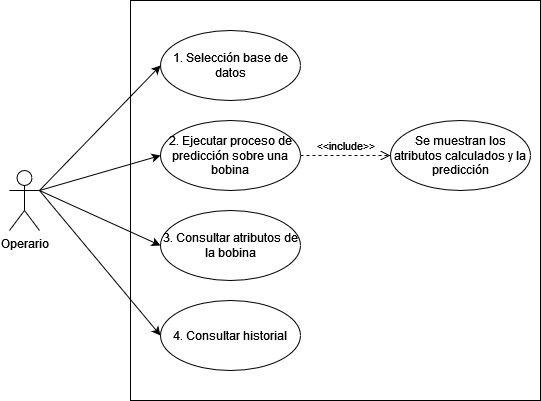
\includegraphics[width=1\textwidth]{img/casosUso.png}
 \caption{Diagrama de Casos de Uso}
 \label{f:casus}
\end{figure}

\newpage
\subsection{Especificación de casos de uso}
A continaucón se muestra una tabla para cada caso de uso:

\begin{center}
\begin{tabular}{|ll|}
\hline
\multicolumn{2}{|l|}{\textbf{CU 1 - Selección base de datos}}                                                                                                                                                          \\ \hline
\multicolumn{1}{|l|}{\textbf{Descripción}}     & \begin{tabular}[c]{@{}l@{}}Permite al operario seleccionar los diferentes valores que \\ permitan conectarse a la base de datos para cargar los valores.\end{tabular} \\ \hline
\multicolumn{1}{|l|}{\textbf{Requisitos}}      & REQ 1.1                                                                                                                                                               \\ \hline
\multicolumn{1}{|l|}{\textbf{Precondiciones}}  & Se está ejecutando el notebook de la aplicación.                                                                                                                      \\ \hline
\multicolumn{1}{|l|}{\textbf{Secuencia}}       & \begin{tabular}[c]{@{}l@{}}1. El usuario rellena los campos: user, password, host y \\ database \\ 2. El usuario ejecuta la celda correspondiente\end{tabular}            \\ \hline
\multicolumn{1}{|l|}{\textbf{Postcondiciones}} & La celda se ejecuta bien y aparece un 2 a su izquierda                                                                                                                \\ \hline
\multicolumn{1}{|l|}{\textbf{Excepciones}}     & \begin{tabular}[c]{@{}l@{}}Se introducen los valores de forma incorrecta y sin el formato \\ necesario en Python y salta un error\end{tabular}                        \\ \hline
\end{tabular}
\captionof{table}{Caso de Uso - 1}
\label{t:caso1}
\end{center}

\begin{center}
\begin{tabular}{|ll|}
\hline
\multicolumn{2}{|l|}{\textbf{CU 2 - Ejecución proceso de predicción sobre una bobina}}                                                                                                                                                                                                                                \\ \hline
\multicolumn{1}{|l|}{\textbf{Descripción}}     & \begin{tabular}[c]{@{}l@{}}Permite al operario seleccionar la ID de la bobina desea\\ sobre la que calcular las predicciones.\end{tabular}                                                                                                                           \\ \hline
\multicolumn{1}{|l|}{\textbf{Requisitos}}      & REQ 1.2, REQ 1.3 y REQ 1.4                                                                                                                                                                                                                                           \\ \hline
\multicolumn{1}{|l|}{\textbf{Precondiciones}}  & \begin{tabular}[c]{@{}l@{}}Se está ejecutando el notebook de la aplicación, y se\\ ha indicado la base de datos.\end{tabular}                                                                                                                                        \\ \hline
\multicolumn{1}{|l|}{\textbf{Secuencia}}       & \begin{tabular}[c]{@{}l@{}}1. El usuario ejecuta la tercera celda.\\ 2. El usuario selecciona en el desplegable la ID de la\\ bobina.\\ 3. El usuario observa los valores y predicciones mostradas\\ por pantalla, y decide si seleccionar otra bobina.\end{tabular} \\ \hline
\multicolumn{1}{|l|}{\textbf{Postcondiciones}} & \begin{tabular}[c]{@{}l@{}}Se muestran los atributos calculados de la bobina y \\ la decisión del modelo.\end{tabular}                                                                                                                                               \\ \hline
\multicolumn{1}{|l|}{\textbf{Excepciones}}     & \begin{tabular}[c]{@{}l@{}}Se produce algún problema durante el proceso y el \\ modelo devuelve algún error.\end{tabular}                                                                                                                                            \\ \hline
\end{tabular}
\captionof{table}{Caso de Uso - 2}
\label{t:caso2}
\end{center}

\begin{center}
\begin{tabular}{|ll|}
\hline
\multicolumn{2}{|l|}{\textbf{CU 3 - Consultar atributos de la bobina}}                                                                                                                                                                                                                  \\ \hline
\multicolumn{1}{|l|}{\textbf{Descripción}}     & \begin{tabular}[c]{@{}l@{}}Permite al operario conocer los atributos y el mapa\\ codificado de la bobina previamente calculados.\end{tabular}                                                                                          \\ \hline
\multicolumn{1}{|l|}{\textbf{Requisitos}}      & REQ 2.1                                                                                                                                                                                                                                \\ \hline
\multicolumn{1}{|l|}{\textbf{Precondiciones}}  & Se ha realizado una predicción sobre la bobina deseada.                                                                                                                                                                                \\ \hline
\multicolumn{1}{|l|}{\textbf{Secuencia}}       & \begin{tabular}[c]{@{}l@{}}1. El usuario se dirige a la ruta donde se encuentra\\ la aplicación.\\ \\ 2. El usuario se dirige al directorio /bobinas.\\ 3. El usuario abre el CSV correspondiente a la \\ bobina deseada.\end{tabular} \\ \hline
\multicolumn{1}{|l|}{\textbf{Postcondiciones}} & \begin{tabular}[c]{@{}l@{}}El usuario consigue abrir el fichero correctamente, y\\ en su interior se encuentran todos los atributos.\end{tabular}                                                                                      \\ \hline
\multicolumn{1}{|l|}{\textbf{Excepciones}}     & -                                                                                                                                                                                                                                      \\ \hline
\end{tabular}
\captionof{table}{Caso de Uso - 3}
\label{t:caso3}
\end{center}

\begin{center}
\begin{tabular}{|ll|}
\hline
\multicolumn{2}{|l|}{\textbf{CU 4 - Consultar el historial}}                                                                                                                                                  \\ \hline
\multicolumn{1}{|l|}{\textbf{Descripción}}     & \begin{tabular}[c]{@{}l@{}}Permite al operario poder revisar el historial de las\\ diferentes predicciones realizadas.\end{tabular}                          \\ \hline
\multicolumn{1}{|l|}{\textbf{Requisitos}}      & REQ 2.2 y REQ 3                                                                                                                                              \\ \hline
\multicolumn{1}{|l|}{\textbf{Precondiciones}}  & \begin{tabular}[c]{@{}l@{}}Se ha realizado al menos una predicción sobre\\ cualquier bobina.\end{tabular}                                                    \\ \hline
\multicolumn{1}{|l|}{\textbf{Secuencia}}       & \begin{tabular}[c]{@{}l@{}}1. El usuario se dirige a la ruta donde se encuentra\\ la aplicación.\\ 2. El usuario sabre el archivo historial.txt\end{tabular} \\ \hline
\multicolumn{1}{|l|}{\textbf{Postcondiciones}} & \begin{tabular}[c]{@{}l@{}}El archivo contiene en su interior los resultados\\ previamente calculados.\end{tabular}                                          \\ \hline
\multicolumn{1}{|l|}{\textbf{Excepciones}}     & -                                                                                                                                                            \\ \hline
\end{tabular}
\captionof{table}{Caso de Uso - 4}
\label{t:caso4}
\end{center}
\apendice{Especificación de diseño}

\section{Introducción}

\section{Diseño de datos}

\section{Diseño procedimental}

\section{Diseño arquitectónico}



\apendice{Documentación técnica de programación}

\section{Introducción}
Este cuarto apéndice va destinado a las personas dedicadas a la informática y que quieran seguir con el proyecto en el futuro. Es por ello, que es necesario explicar todo claramente para que se pueda comprender. Los temas sobre los que se va a tratar son: estructura de directorios, manual del programador, ejecución del proyecto y pruebas del sistema.

\section{Estructura de directorios}
Este subapartado contiene la información sobre la estructura del proyecto, junto con sus diferentes directorios y ficheros. Además, toda la estructura se puede ver de manera pública en el repositorio de GitHub\footnote{Repositorio: \url{https://github.com/ifh1001/TFM}} del proyecto. A continuación, se puede ver de manera gráfica:
\dirtree{%
.1 /.
.2 \texttt{doc}.
.2 \texttt{src}.
.2 \texttt{LICENSE}.
.2 \texttt{README.md}.
.2 \texttt{requirements.txt}.
}
Como se aprecia, se distinguen del directorio raíz 5 elementos, que se van a explicar a continuación:
\begin{itemize}
    \item \textbf{doc:} contiene toda la información relacionada con la documentación.
    \item \textbf{src:} contiene en su interior todo el código desarrollado a lo largo del proyecto. Además, contiene la aplicación, junto con todo lo necesario para que pueda usarse.
    \item \textbf{LICENSE:} fichero que contiene la licencia del proyecto, que como ya se ha comentado en el primer apéndice, es una licencia de tipo GPL v3.
    \item \textbf{README.md:} contiene una breve descripción del repositorio, con el fin de que el lector comprenda la finalidad del proyecto.
    \item \textbf{requirements.txt:} fichero que reúne los requisitos necesarios de librerías y versiones para ejecutar sin ningún problema la aplicación.
\end{itemize}

\subsection{Documentación}
Como se ha comentado previamente, la documentación se encuentra en el directorio \texttt{/doc}. En él se encuentra un conjunto de ficheros escritos en \LaTeX que si se compilan todos ellos juntos se obtiene la memoria en formato PDF que da lugar a esta memoria que se está leyendo.

\subsection{Código}
El código desarrollado en el proyecto se encuentra en el directorio \texttt{/src}. A continuación se muestra la división de directorios y ficheros del mismo:
\dirtree{%
.1 \texttt{/src/}.
.2 \texttt{aplicacion}.
.3 \texttt{modelos}.
.3 \texttt{Aplicacion.ipynb}.
.3 \texttt{funciones.py}.
.2 \texttt{CargaDatos.ipynb}.
.2 \texttt{EvaluacionCNNs.ipynb}.
.2 \texttt{ObtencionCaracteristicas.ipynb}.
.2 \texttt{PreparacionCNNs.ipynb}.
.2 \texttt{VisualizacionDatos.ipynb}.
}

Como se puede apreciar, el directorio \texttt{/src} está formado por un directorio y cinco \emph{notebooks}. A continuación, se puede ver una explicación sobre cada uno:

\begin{itemize}
    \item \texttt{aplicacion:} en este directorio se encuentra la estructura necesaria para que funcione la aplicación. Como se puede ver, hay un directorio más, \texttt{/modelos}, donde se encuentran almacenados los cinco modelos que utilizará la aplicación. Además, hay dos ficheros, un \emph{notebook} que será la aplicación y un fichero de \emph{Python} que contiene todas las funciones de manera encapsulada para que se pueda utilizar la aplicación de la manera más sencilla posible.
    \item \texttt{CargaDatos.ipynb:} este \emph{notebook} contiene las primeras pruebas que se realizaron sobre los datos para conocer las diferentes tablas y registros que tenía cada una. Además, contiene una evaluación de bobinas según si cumplen o no todas sus tejas, los requisitos de zinc.
    \item \texttt{EvaluacionCNNs.ipynb:} este fichero contiene los diferentes experimentos que se han llevado a cabo para obtener él mejore conjunto de modelos con la mayor precisión. Además, también guarda todos los modelos obtenidos para poder emplear cualquiera.
    \item \texttt{ObtencionCaracteristicas.ipynb:} este \emph{notebook} se encarga de obtener el mapa codificado de cada bobina junto con las diferentes \emph{features}. Todos estos datos se calculan para cada tipo de datos, 1D y 2D, y para cada uno de los diferentes sensores.
    \item \texttt{PreparacionCNNs.ipynb:} este fichero contiene las diferentes pruebas que se han efectuado para aprender a construir modelos con \emph{tensorflow} para familiarizarse con la librería y sentirse cómodo con el uso de la misma.
    \item \texttt{VisualizacionDatos.ipynb:} contiene una visualización de los valores de zinc para cada bobina en forma de gráfica, para cada uno de los sensores de los datos 1D.
\end{itemize}

\section{Manual del programador}
Tal y como se acaba de ver en el subpunto anterior. La aplicación se encuentra en el directorio \texttt{/src/aplicacion}. En él se pueden implementar nuevas funcionalidades de la aplicación añadiéndolas al fichero \texttt{funciones.py}. Además, en su interior, se encuentran todas las funciones debidamente comentadas para que puedan ser comprendidas y mejoradas en caso de que se desee. Adicionalmente, si se consiguen mejores modelos se pueden eliminar los antiguos y añadir los nuevos en el directorio \texttt{/src/aplicacion/modelos}.

Si se quiere realizar alguna prueba más sobre las redes neuronales, o construir algunas nuevas empleando diferentes estrategias, o incluso utilizando datos diferentes, mi recomendación es que se realice en un \emph{notebook}, usando por ejemplo \emph{Jupyter Notebook}, ya que permite visualizar todo de una manera mucho más sencilla y posteriormente exportar las funciones a un fichero de \emph{Python}. Todos estos nuevos ficheros se pueden añadir directamente al directorio raíz del código (\texttt{/src}).

\section{Compilación, instalación y ejecución del proyecto}
Para usar la aplicación desarrollada en el proyecto, es necesario tener instalado en el dispositivo un entorno que tenga todas las dependencias de librerías que usa la aplicación, junto con una herramienta que permita ejecutar \emph{notebooks}, siendo recomendad el uso de \emph{Jupyter Notebook}.

Las librerías utilizadas se pueden ver a continuación:
\begin{itemize}
    \item MySQL
    \item Pandas
    \item NumPY
    \item Jupyter Widgets
    \item TensorFlow
\end{itemize}

De forma que al instalar todas ellas en un entorno, se podría ejecutar sin ningún problema la aplicación. Pese a todo, y por si en algún punto existen versiones incompatibles entre sí, en el repositorio de GitHub existe el fichero \texttt{requirements.txt} para que se puedan instalar en un entorno de Anaconda las versiones utilizadas en el proyecto que garantizarían el correcto empleo de la aplicación. Dicho fichero se puede encontrar en el siguiente enlace:

\url{https://github.com/ifh1001/TFM/blob/main/requirements.txt}

Una vez se cuenten con las librerías instaladas, se puede usar la aplicación. Para ello, con una herramienta que permita ejecutar \emph{notebooks} se puede abrir el correspondiente a la aplicación y ejecutar las tres celdas que la componen para poder seleccionar las bobinas sobre las que realizar predicciones.

\section{Pruebas del sistema}
Este proyecto se ha centrado en la investigación de obtener un grupo de modelos capaces de predecir si una bobina iba a ser válida o no para poder usarse por parte de la empresa. Es por ello, que se ha dado más peso a la investigación que a la construcción de una aplicación lo más perfecta posible y realizando pruebas de sistema para garantizar su correcto funcionamiento.

Pese a todo, se han llevado a cabo dos pruebas relevantes a la hora de construir y evaluar los modelos. Por un lado, se han separado del conjunto de datos inicial, una muestra de bobinas para, tras construir los modelos, evaluarlos con datos que nunca habían visto y así obtener unos resultados lo más realistas y probables posibles.

Por otro lado, se llevó a cabo una prueba para obtener el mejor criterio de clasificación, probando un total de 6 valores, y para cada uno de ellos calcular y representar la curva ROC junto con su AUC, de forma, que se ha trabajado con aquel que mejor AUC tenía, ya que este criterio es él más óptimo para separar las clasificaciones entre una clase u otra.
\apendice{Documentación de usuario}

\section{Introducción}
En este último apéndice, se incluye la información necesaria para poder utilizar la aplicación del proyecto, como poder instalarlo y el manual de usuario para saber utilizar la aplicación.

\section{Requisitos de usuarios}
El primer requisito por parte del usuario es la necesidad de tener conexión a Internet, ya que los datos se encuentran alojados en una base de datos, por lo que para poder usarla será necesario tener conexión.

En segundo lugar, necesitará tener un entorno con todas las librerías que usa la aplicación, junto con alguna aplicación que permite ejecutar un \emph{notebook}, como, por ejemplo, \emph{Jupyter Notebook}.

Una vez se diponga de todo lo anterior, ya sería posible poder utilizar la aplicación que se ha llevado a cabo en este proyecto.

\section{Instalación}
En primer lugar, sería necesario descargar en instalar Anaconda en caso de que no se disponga de dicha herramienta, ya que permite crear un entorno con todos los requisitos de la aplicación, permitiendo que se pueda usar sin ningún problema. Para ello, es tan sencillo como ir a la siguiente ruta:

\url{https://www.anaconda.com/download}

Y en ella descargar la versión adecuada a tu sistema operativo. Tras esto, sería tan sencillo como seguir el instalador y esperar unos minutos a que termine la instalación.

En segundo lugar, habría que instalar las dependencias de la aplicación. Para facilitar este proceso se ha dejado en el repositorio del proyecto un fichero \emph{requirements}, obtenido de un entorno \emph{Windows}, que permitirá descargar todas las librerías junto con sus versiones que hacen que se garantice la posibilidad de utilizar la aplicación. Dicho fichero se puede encontrar en el siguiente enlace:

\url{https://github.com/ifh1001/TFM/blob/main/requirements.txt}

En tercer, y último lugar, para poder instalar las dependencias, se abrirá la consola \emph{Anaconda Prompt} y se escribirá el siguiente comando:

\begin{verbatim}
conda create --name nombre_entorno --file requirements.txt
\end{verbatim}

Y tras esperar unos minutos, se habrán instalado todas las dependencias, por lo que ya se ha creado un entorno que sea capaz de lanzar la aplicación.

\section{Manual del usuario}
En primer paso para poder utilizar la aplicación, es lanzar \emph{Jupyter Notebook}. Para ello, y basándose en el apartado de instalación, lo primero sería cambiar al nuevo entorno, y posteriormente ejecutar el comando de la herramienta. Ambos comandos se muestran a continuación:

\begin{verbatim}
    conda activate nombre_entorno
    
    jupyter notebook
\end{verbatim}

Tras su ejecución aparecerá en el navegador la herramienta, y sería tan sencillo como dirigirse al directorio donde se encuentra el \emph{notebook} de la aplicación. Tras abrirlo se verá que hay 3 celdas y que habrá que ejecutar en orden. Para ejecutar una celda, hacemos clic sobre ella y pulsamos al botón \textbf{Run} que se encuentra en el menú superior, tras esperar un rato veremos como a la izquierda de la celda aparecerá un 1, de igual forma que se puede ver en la Figura \ref{f:celda1}.

\begin{figure}[h]
 \centering
  
\includegraphics[width=0.7\textwidth]{img/celda1.PNG}
 \caption{Ejecución de la Primera Celda}
 \label{f:celda1}
\end{figure}

A continuación, será necesario ejecutar la segunda celda, o previamente modificar los valores en caso de que se quiera utilizar una base de datos diferente a la que viene por defecto. Tras su ejecución aparecerá a la izquierda un 2.

Finalmente, se ejecutará la última celda, y se verá como aparece un desplegable que muestra las IDs de todas las bobinas cargadas de la base de datos, Figura \ref{f:celda3}. Sería tan sencillo como seleccionar una y esperar a que aparezcan los resultados. Este proceso se puede repetir tantas veces como se desee, simplemente volviendo a seleccionar otra bobina desde el desplegable.

\begin{figure}[h]
 \centering
  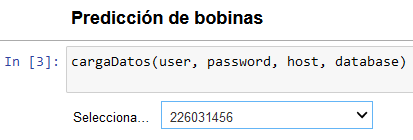
\includegraphics[width=0.7\textwidth]{img/celda3.PNG}
 \caption{Ejecución de la Tercera Celda}
 \label{f:celda3}
\end{figure}

También, en el directorio \texttt{./bobinas} se verán los diferentes CSV asociados a las bobinas sobre las que se han realizado predicciones. Además, junto al \emph{notebook} de la aplicación, se encontrará el fichero historial.txt donde se podrá consultar las predicciones de todas las bobinas.

Tras usar la aplicación, sería tan sencillo como cerrar la pestaña de la aplicación y finalmente cerrar la consola desde la que se ha lanzado \emph{Jupyter Notebook}, y de esta forma se detendría todo el proceso por completo.


\bibliographystyle{plain}
\bibliography{bibliografia}

\end{document}
